\documentclass[12pt]{article}
\usepackage[margin=1in]{geometry}
\usepackage{amsmath, amssymb}
\usepackage{graphicx}
\usepackage{hyperref}
\usepackage{enumitem}
\usepackage{titlesec}
\usepackage{fancyhdr}
\usepackage{tikz}
\usetikzlibrary{arrows.meta, positioning}

\pagestyle{fancy}
\fancyhf{}
\rhead{Checkpoint 2: Technical Summary}
\lhead{CS 498 (Spring 2024)}
\rfoot{Page \thepage}

\titleformat{\section}{\normalfont\Large\bfseries}{\thesection}{1em}{}
\titleformat{\subsection}{\normalfont\large\bfseries}{\thesubsection}{1em}{}

\title{Technical Summary Report: \\ A Linear-Time Algorithm for Linearizing Higher-Order Shortest Path Problems}
\author{Muhammad Hassaan Tariq \\ Rohaan Ahmed\\
\texttt{mt08081@st.habib.edu.pk}\\
\texttt{ra08102@st.habib.edu.pk}\\
Habib University}
\date{April 2024}

\begin{document}
\maketitle

\section{Problem and Contribution}

The paper \textit{“A linear time algorithm for linearizing quadratic and higher-order shortest path problems”} by Çela et al. addresses the \textbf{linearization problem} for the \textbf{Quadratic Shortest Path Problem (QSPP)} and its generalizations to order-$d$ shortest path problems (SPP$_d$). While the classical Shortest Path Problem (SPP) is polynomially solvable, the QSPP is known to be NP-hard even under specific restrictions (e.g., adjacent arcs).

The central contribution of the paper is a novel algorithm that:
\begin{itemize}[itemsep=2pt]
    \item Tests linearizability of QSPP/SPP$_d$ instances on acyclic digraphs.
    \item Runs in \textbf{linear time} relative to the input size for fixed $d$.
    \item Provides a \textbf{constructive linearizing cost function} when linearization is possible.
    \item Computes a basis of all linearizable instances, which is useful for deriving tighter lower bounds in exact algorithms.
\end{itemize}

This contribution is significant because it reduces a globally complex problem to a series of efficiently checkable local conditions.

\section{Algorithmic Description}

\subsection*{Inputs and Outputs}
\begin{itemize}
    \item \textbf{Input:} An acyclic digraph $G = (V, A)$ with distinguished source $s$ and sink $t$, and a cost function $f$ defined on arc subsets of size $d$.
    \item \textbf{Output:} Either a linearizing function $c : A \to \mathbb{R}$ such that the nonlinear path costs can be reproduced using $c$, or a certificate that no such $c$ exists.
\end{itemize}

\subsection*{How the Algorithm Works: Checking and Simplifying Path Costs}

Imagine you're trying to find the ``best'' route on a map, but the cost isn't straightforward like just adding up distances. Maybe the cost depends on which roads you take together---this is similar to the \textit{Quadratic Shortest Path Problem}. The big goal is to determine whether we can simplify this complex cost structure. Specifically, can we assign a simple cost to each individual road such that the total cost of any route is just the sum of these individual costs? If yes, we say the problem is \textbf{linearizable}—it can be transformed into a standard, easier-to-solve shortest path problem.

\subsubsection*{Focus on Small Sections (Two-Path Systems)}

Rather than analyzing the entire map at once, the algorithm examines smaller structures. Consider any city $v$ on the map. Identify two paths from the start city $s$ to $v$ (denoted $P_1$ and $P_2$) and two paths from $v$ to the end city $t$ (denoted $Q_1$ and $Q_2$). This yields four complete paths from $s$ to $t$ that all go through $v$: $P_1Q_1$, $P_2Q_2$, $P_1Q_2$, and $P_2Q_1$. This configuration is called a \textit{two-path system}.

\subsubsection*{The Local Check (The Equation)}

For each two-path system, the algorithm verifies a consistency condition using the original cost function $f$. The check involves the following equation:
\[
f(P_1Q_1) + f(P_2Q_2) = f(P_1Q_2) + f(P_2Q_1)
\]
In simpler terms, this equation asks whether the cost behaves predictably when we swap the suffixes ($Q_1$, $Q_2$) between the prefixes ($P_1$, $P_2$). If the equation holds, the cost function $f$ is acting in a way that suggests the existence of an equivalent additive cost representation.

\subsubsection*{Algorithm Step 1: Test Everywhere}

The first phase of the algorithm systematically applies this equation to all relevant two-path systems across the map. Although optimizations may reduce the number of checks, the algorithm ensures complete coverage. If even one instance of the equation fails, the algorithm halts and concludes that the problem is \textbf{not linearizable}.

\subsubsection*{Algorithm Step 2: Build the Simple Costs (If Possible)}

If the equation passes for all examined systems, the problem is linearizable. The next step is to compute the additive cost $c$ for each road. The algorithm accomplishes this by processing the cities in topological order (which is applicable since the map contains no cycles). Starting from pre-defined costs on certain \textit{nonbasic arcs}, the algorithm deduces a unique additive cost for every other arc in the graph. This results in a transformed, simplified shortest path problem using only linear costs.

\begin{figure}[h]
\centering
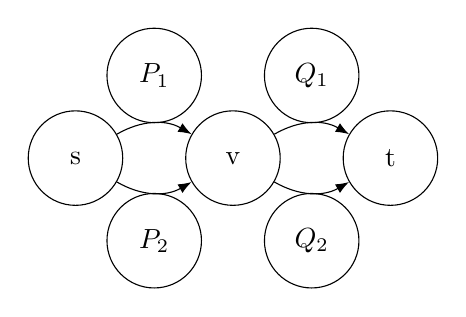
\begin{tikzpicture}[node distance=2cm, on grid, auto, every node/.style={circle, draw, minimum size=1.2cm}]
    \node (s) {s};
    \node (v) [right=of s] {v};
    \node (t) [right=of v] {t};
    \path[-{Latex}] (s) edge[bend left] node[above] {$P_1$} (v);
    \path[-{Latex}] (s) edge[bend right] node[below] {$P_2$} (v);
    \path[-{Latex}] (v) edge[bend left] node[above] {$Q_1$} (t);
    \path[-{Latex}] (v) edge[bend right] node[below] {$Q_2$} (t);
\end{tikzpicture}
\caption{Two-path system used to test local linearizability}
\end{figure}

\section{Comparison with Previous Approaches}

Previous algorithms for testing linearizability, especially for the QSPP, had time complexity $O(nm^3)$ or higher. The algorithm proposed in this paper:
\begin{itemize}[itemsep=2pt]
    \item Has linear time complexity for fixed $d$ (e.g., $O(m^2)$ for QSPP).
    \item Avoids global combinatorial checks by reducing the problem to a localized algebraic identity.
    \item Exploits graph structure (e.g., topological orderings of acyclic graphs) and dynamic programming for efficient computation.
\end{itemize}

\section{Data Structures and Techniques}

\begin{itemize}[itemsep=2pt]
    \item \textbf{Graph Representation:} Acyclic digraphs are processed using topological sort to ensure linear traversal.
    \item \textbf{Dynamic Programming:} Used to solve APECP$_1$ (All Paths Equal Cost Problem) instances.
    \item \textbf{In-trees:} Nonbasic arcs are chosen to form in-trees rooted at $t$, simplifying the cost propagation.
    \item \textbf{Linear Algebra:} The space of linearizable cost functions is characterized as a subspace; a basis is computed.
    \item \textbf{Auxiliary Variables:} $\gamma$ values are computed to optimize recursive decomposition from SPP$_d$ to SPP$_1$.
\end{itemize}

\section{Implementation Outlook}

\subsection*{Feasibility}
The algorithm is well-structured and amenable to implementation. The linear time guarantee ensures it scales well for large graphs with small $d$. An elaborate pseudocode is present on \textbf{page 179} of the journal in question. This makes implementing the algorithm quite straightforward and plausible.

\subsection*{Challenges}
\begin{itemize}[itemsep=2pt]
    \item \textbf{Numerical Stability:} Summing path costs may introduce rounding errors.
    \item \textbf{Edge Cases:} Degenerate two-path systems or shared arcs must be handled carefully.
    \item \textbf{Memory Efficiency:} Higher-order terms may require careful storage and reuse to stay within space limits.
\end{itemize}


\end{document}
